\section{提案手法} \label{sec4}
本章では，五つのコンポーネントから構成される提案手法について述べる．提案手法は，LLMとシミュレータから取得した家庭環境知識を用いて，タスクを実行するためのアクションを逐次的に生成する．さらに，LLMを用いて生成されたアクションの前提条件を検証し，違反と判定した場合には代替アクションを1回再生成する．提案手法の構成図を~\ref{proposed_method}に示す．以下の詳細仕様は公開された\texttt{single-prompt.ipynb}および\texttt{multi-prompts.ipynb}のコードに基づく．このコードと過去の全実験条件との対応については\ref{sec5.provenance}に制約を述べる．

\begin{figure}[t]
  \begin{center}
    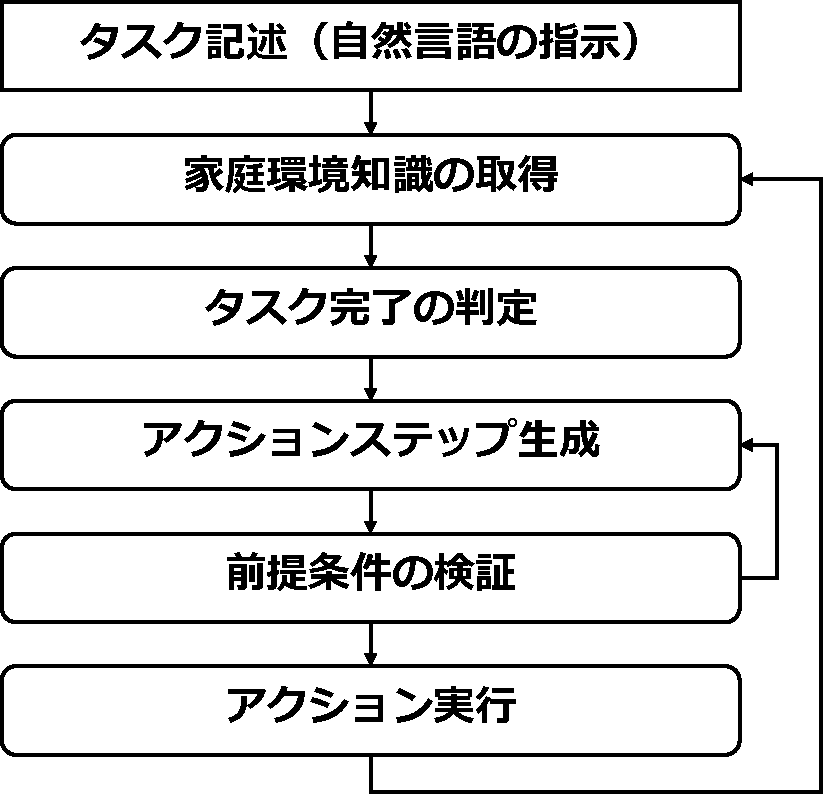
\includegraphics[width=8cm]{figures/proposed_method.pdf}
    \caption{提案手法の構成．図は処理の概略を表し，終了判定・上限判定の順序はAlgorithm~\ref{alg:public_run}に従う．}
    \label{proposed_method}
  \end{center}
\end{figure}


\subsection{家庭環境知識の取得} \label{sec4.1}
\ref{proposed_method}の「家庭環境知識の取得」では，シミュレータのグラフをコードで抽出・自然言語化する．この抽出処理自体にLLMは用いない．まずspaCyの\texttt{en\_core\_web\_sm}でタスク文を解析し，品詞がNOUNの語と\texttt{inflection.singularize}による単数形候補を取得する．次に，その語集合に\texttt{class\_name}が一致する物体ノードを家屋全体から選ぶ．文字列一致による選択であり，同義語検索や指示中の修飾関係の解析は行わない．

選択した物体について，状態配列と，出辺のON・INSIDEを走査する．INSIDEの相手が\texttt{bathroom, bedroom, kitchen, livingroom}のいずれかなら所属部屋として扱い，それ以外なら容器として扱う．ONの相手は支持物として扱うが，相手クラスが\texttt{walk}または\texttt{floor}の場合は除外する．\texttt{walk}は公開コード中の文字列をそのまま記したものである．支持物・容器を追加対象として一度だけ展開し，その状態・支持／包含関係・所属部屋を読む．追加対象からさらにノード集合を再帰的に拡張する処理はない．また，既に選択済みのノードが追加対象にも現れると，そのノードの記録を初期化して再走査する．各ON・INSIDE・所属部屋の格納欄は単一値であり，複数の同種関係はグラフの走査順に上書きされる．

エージェントについては，ID 1の出辺から所属部屋，左右の手の保持物，抽出対象へのCLOSE関係を取得する．エージェントのノード状態配列は自然言語化していない．物体が保持する対象の列挙も，走査時の抽出集合に含まれる物体に限られ，全内容物の列挙ではない．

自然言語化では物体名とID，状態配列の先頭要素，ONまたはINSIDE関係，所属部屋を文章にする．ONとINSIDEの両方がある場合はONを優先する．所属部屋を得られない物体では基本の説明文を出力せず，保持対象の列挙があればその部分のみを出力する．保持対象が容器の中か支持物の上かは\texttt{CONTAINERS}属性の有無で記述する．このため，シミュレータの完全なグラフを取得できることと，計画器に必要な全情報が提示されることは同義ではない．位置座標，画像，壁面や床面の任意の関係は入力しない．正確な変換関数と説明用入力に対する出力例は\ref{app:knowledge}に示す．


\subsection{タスク完了の判定} \label{sec4.2}
\begin{figure*}[tb]
    \begin{lstlisting}[caption=「タスク完了の判定」で用いるプロンプトテンプレート, label=prompt1]
The current states in the home are as follows: 
@\textcolor{red}{\textit{[ Home environment knowledge ]}}@

If the following task has already completed based on the current status, output "End"; otherwise, output "Continue".
Task: @\textcolor{red}{\textit{[ Task description ]}}@
    \end{lstlisting}
\end{figure*}

\begin{figure*}[tb]
    \begin{lstlisting}[caption=「アクションステップ生成」で用いるプロンプトテンプレート, label=prompt2]
You need to generate a next action step for completing a household task.

Allowed actions: @\textcolor{red}{\textit{[ Allowed actions ]}}@
Output format: @\textcolor{red}{\textit{[ Output format ]}}@

Example Task: @\textcolor{red}{\textit{[ An example Task ]}}@
@\textcolor{red}{\textit{[ Action plan for the example task ]}}@

The current states in the home are as follows: 
@\textcolor{red}{\textit{[ Home environment knowledge ]}}@

Generate a only next action step to complete the following task and output only that.
Task: @\textcolor{red}{\textit{[ Task description ]}}@
Step1:
    \end{lstlisting}
\end{figure*}

\ref{proposed_method}の「タスク完了の判定」では，LLMが家庭環境知識に基づき，タスクが完了しているかを判定する．

Listing~\ref{prompt1}はMulti Promptsにおける入力の内容を示す．実装では環境知識に終了判定文を連結し，systemメッセージと一つのuserメッセージで問い合わせる．Single Promptでは終了判定文の文面が異なる．両方式の全文と空白・改行を含む組立て規則を\ref{app:prompts}に示す．

出力が文字列``End''と完全一致した場合に通常の採点へ進む．前後の空白を除去する処理はない．参照列長が0の場合は，最初の出力が``End''ならゴールグラフを再確認せず成功，``Continue''なら上限到達による失敗として返す．これ以外の出力に対する専用の再問い合わせ処理はなく，行動生成へ進む．

行動のカウンタは1から開始し，成功実行の後に上限を検査し，上限未満なら1加算する．上限に達した場合は次の完了判定を行わず失敗として返す．したがって，上限ちょうどの行動でゴールに達した場合も成功にはならない．全体の判定順序をAlgorithm~\ref{alg:public_run}に，上限の算出方法を\ref{sec5.2}に示す．


\subsection{アクションステップ生成} \label{sec4.3}

\ref{proposed_method}の「アクションステップ生成」では，LLMと家庭環境知識を用いて，タスクを達成するために必要な次のアクションステップを一つ生成する．

本コンポーネントで用いるプロンプトテンプレートをListing~\ref{prompt2}に示す．本プロンプトテンプレートは，「実行可能なアクションとその出力形式（Listing~\ref{prompt2}の3行目と4行目）」，「One-shot学習用の例（タスクと行動計画）（Listing~\ref{prompt2}の6行目と7行目）」，「家庭環境知識（Listing~\ref{prompt2}の10行目）」，「タスクとアクションの実行履歴（Listing~\ref{prompt2}の13，14行目）」の四つの要素から構成される．

これらに冒頭の役割指示を加えた5要素を，Single Promptでは一つのuserメッセージに連結し，Multi Promptsでは順序を保った五つのuserメッセージとして渡す．どちらも，次の行動を生成する呼び出しは1回である．Multi Promptsは，要素ごとにLLMの応答を得てから次を提示する方式ではない．各周回で更新した環境知識と，それまでに実行成功した行動履歴からメッセージを作り直す．修正前の候補行動や過去の前提条件判定は次周回の実行履歴には追加しない．

事例検索には\texttt{sentence-transformers/all-MiniLM-L6-v2}を用いる．事例集合の異なるタスク名を埋め込み，入力タスク名とのコサイン類似度が最大の1名を選ぶ．同名の事例が複数ある場合は最長の参照行動列を採択する．長さ同点はJSON中で先に現れる事例を選ぶ．検索の候補名は公開コードで\texttt{set}からリストへ変換されるため，類似度同点時の候補順序は固定されていない．シーン，初期状態，ゴールIDは検索に用いない．



\subsection{前提条件の検証} \label{sec4.4}
\begin{figure*}[tb]
  \begin{center}
    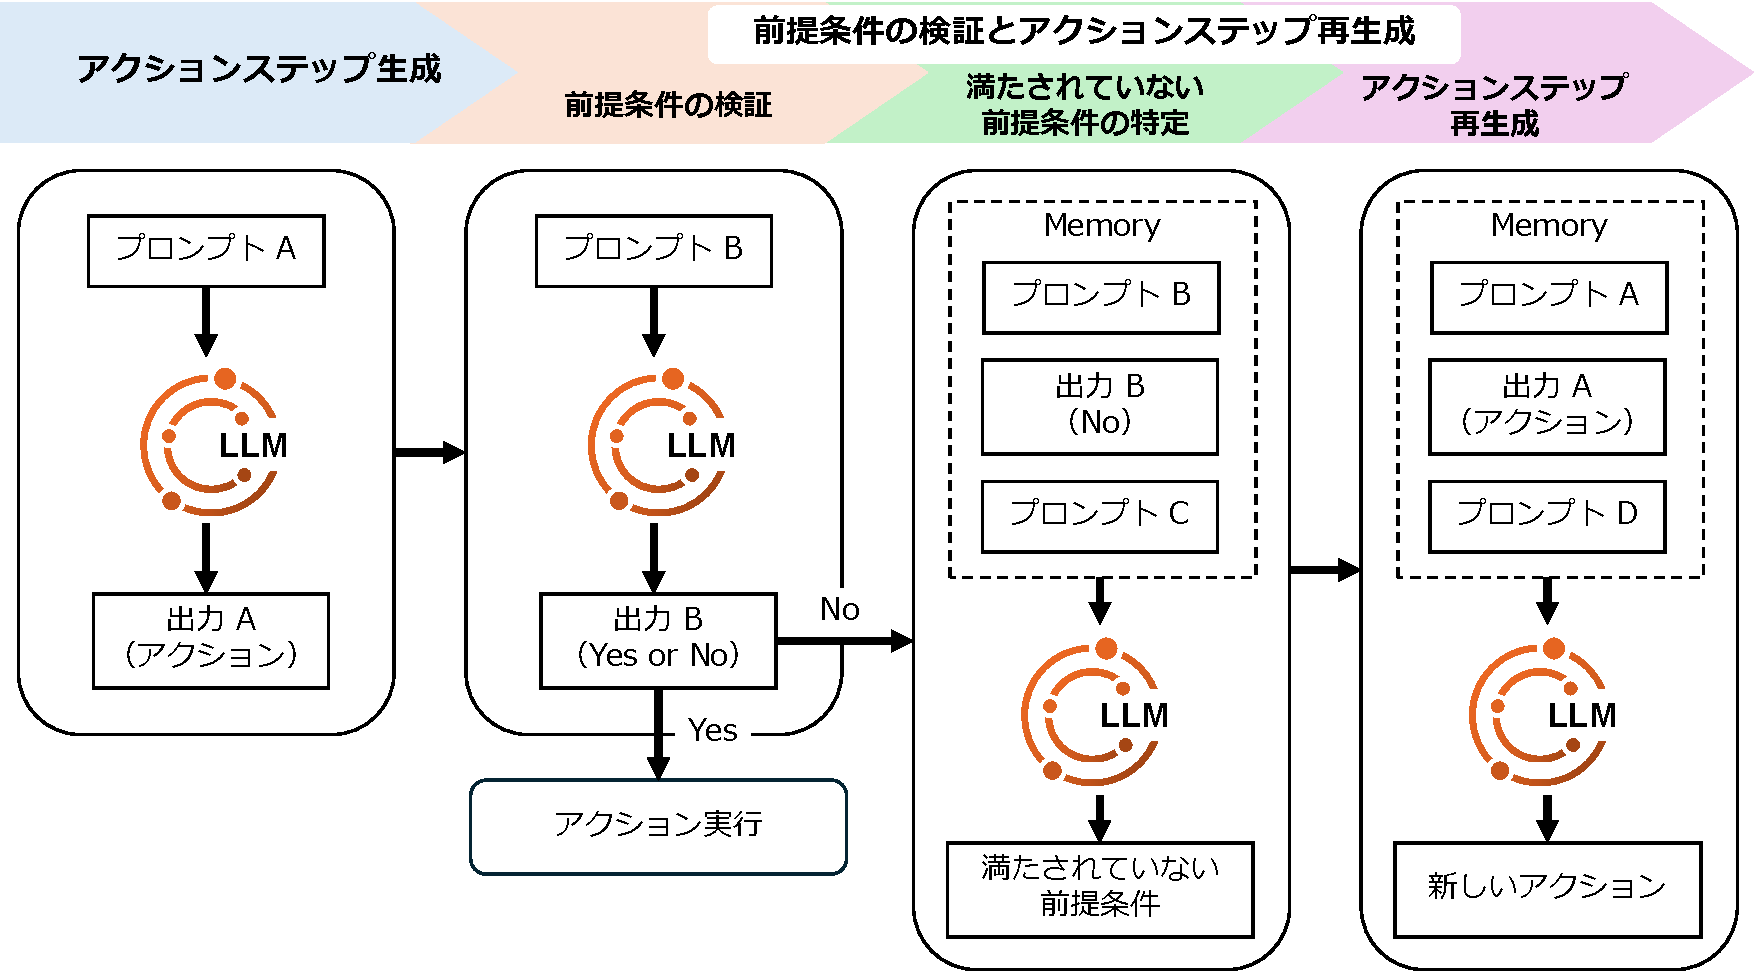
\includegraphics[width=\textwidth]{figures/Precheck.pdf}
    \caption{前提条件の検証とアクションステップ再生成の概要．公開実装は再生成を1回行い，再生成後の行動は再検証せず実行する．}
    \label{Precheck}
  \end{center}
\end{figure*}

\begin{figure*}[tb]
    \begin{lstlisting}[caption=\ref{Precheck}の「前提条件の検証」における「プロンプトB」の生成に用いるプロンプトテンプレート, label=prompt3]
The current states in the home are as follows: 
@\textcolor{red}{\textit{[ Home environment knowledge ]}}@

If the current status satisfies the preconditions, output "Yes"; otherwise, output "No".
Preconditions: @\textcolor{red}{\textit{[ Preconditions ]}}@
    \end{lstlisting}
\end{figure*}

\begin{figure*}[tb]
    \begin{lstlisting}[caption={\ref{Precheck}の「満たされていない前提条件の特定」における「プロンプトC」の生成に用いるプロンプトテンプレート}, label=prompt4]
Which the preconditions are not satisfied?
Output only that.
Preconditions: @\textcolor{red}{\textit{[ Preconditions ]}}@
    \end{lstlisting}
\end{figure*}

\ref{proposed_method}の「前提条件の検証」では，LLMを用いて，生成されたアクションステップを実行するための前提条件を，現在の状況が満たしているかどうかを検証する．さらに，前提条件を満たしていなかった場合には，満たされていない前提条件を特定し，それに基づいてアクションステップの再生成を行う．一連のプロセスの概要を~\ref{Precheck}に示す．

初めに，Listing~\ref{prompt3}の環境知識，判定指示，前提条件文を一つのuserメッセージで与える．この呼び出しにsystemメッセージは付けない．前提条件文は\texttt{precondition.json}から操作名をキーとして選び，対象名・IDを代入する．公開コードは出力に大文字小文字を区別した部分文字列``Yes''が含まれれば充足とし，それ以外は違反条件の特定へ進む．厳密な二値応答の検証ではない．違反条件の特定には判定時のuser入力とassistant出力を履歴として与え，Listing~\ref{prompt4}の問い合わせを追加する．実際の連結では``Output only that.''と条件文の間に改行を追加しない．

違反条件の特定後は，Listing~\ref{prompt5}の内容で再生成を行う．行動生成時のuser入力，候補行動のassistant出力，違反理由のuser入力を履歴とし，タスク・実行履歴・次のステップ番号を含む指示の``Generate''を``Regenerate''へ置換したuser入力を追加する．前提条件判定用の履歴全体を再生成へ引き継ぐ処理ではない．

操作名が条件辞書にない場合は，違反条件の特定を行わず，形式不正というフィードバックで再生成する．空白区切りの引数解析は単純であり，不正な引数数等による例外を包括的に捕捉する実装ではない．いずれの再生成経路も1回で終了し，得られた行動を再検証せず実行する．従って，すべての実行行動について前提条件充足を保証する機構ではない．

%\capwidth=\linewidth
%\lstinputlisting[caption={「満たされていない前提条件の特定」で用いるプロンプトテンプレート（~\ref{precheck}のプロンプトC）},float=tb,label=prompt4-2]{"./listings/Listing4.txt"}


\begin{figure*}[tb]
    \begin{lstlisting}[caption=\ref{Precheck}の「アクションステップ再生成」における「プロンプトD」の生成に用いるプロンプトテンプレート, label=prompt5]
'@\textcolor{red}{\textit{[ Generated action step ]}}@' can not execute, because it is not satisfied the following precondition.
@\textcolor{red}{\textit{[ Unmet preconditions ]}}@

Regenerate a only next action step to complete the following task and output only that.
Task: @\textcolor{red}{\textit{[ Task description ]}}@
@\textcolor{red}{\textit{[ Action execution history ]}}@
Step n: 
    \end{lstlisting}
\end{figure*}

\subsection{アクション実行} \label{sec4.5}
\ref{proposed_method}の「アクション実行」では，生成したアクションステップをシミュレータ上で実行する．また，実行に成功した場合には，実行したアクションステップを実行履歴として\ref{proposed_method}の「アクションステップ生成」で用いるプロンプトの末尾に追加する．その後「家庭環境知識の取得」を再度行い，処理が終了するまで一連のプロセスを繰り返す．なお，アクションの実行に失敗した場合も処理を終了する．

実装は行動文字列に\texttt{<char0>}を付与し，\texttt{render\_script}を\texttt{find\_solution=False}で呼ぶ．失敗した行動は保存列に追加しない．PreCheckなしのアブレーションは検証と再生成の分岐全体をスキップし，生成行動を直接実行する．

\begin{algorithm*}[tb]
\caption{公開実装の1タスクの処理（正常に解析できる入力について）}\label{alg:public_run}
\begin{algorithmic}[1]
\Require タスクインスタンス$T$，検証使用フラグ$p$
\State シーン$T.scene-1$を初期化し，状態配列を上書きして初期部屋にエージェントを配置
\State 指示中の関連名詞$R$と検索事例$E$を取得
\State $M\gets 2|T.action\_scripts|$，$n\gets1$，成功実行履歴$H\gets[]$
\While{true}
  \State $K\gets\operatorname{Serialize}(\operatorname{Extract}(G,R))$
  \State $c\gets\operatorname{LLMEndCheck}(K,T.task)$
  \If{$c$が文字列Endと完全一致}
    \If{$n=1$かつ$M=0$}
      \State \Return Success，$H$ \Comment{グラフの採点を省略する特例}
    \EndIf
    \State 通常のゴール採点を行い，SuccessまたはErroneous Terminateと$H$を返す
  \ElsIf{$c$がContinueと完全一致，かつ$M=0$}
    \State \Return Reaching Maximum Attempts，$H$
  \EndIf
  \State $a\gets\operatorname{LLMGenerate}(K,T.task,E,H,n)$
  \If{$p$}
    \If{$a$の操作名が条件辞書にない}
      \State $a\gets\operatorname{LLMRegenerate}(a,\text{形式不正},K,T.task,E,H,n)$
    \Else
      \State $q\gets\operatorname{LLMPreCheck}(K,\operatorname{BindConditions}(a))$
      \If{$q$に部分文字列Yesが含まれない}
        \State $u\gets\operatorname{LLMUnmetConditions}(K,q,a)$
        \State $a\gets\operatorname{LLMRegenerate}(a,u,K,T.task,E,H,n)$
      \EndIf
    \EndIf
  \EndIf
  \State $s\gets\operatorname{Execute}(a)$ \Comment{再生成後も再検証しない}
  \If{$s$が成功でない}
    \State \Return Execution Failure，$H$
  \EndIf
  \State $a$を$H$とプロンプト内の実行履歴に追加
  \If{$n\geq M$}
    \State \Return Reaching Maximum Attempts，$H$
  \EndIf
  \State $n\gets n+1$
\EndWhile
\end{algorithmic}
\end{algorithm*}


\subsection{実装} \label{sec4.6}
本節では，提案手法の実装について述べる．
提案手法の実装で用いるシミュレータに必要な機能条件を以下に示す．

\begin{itemize}
    \item シミュレータの内部データとして，完全な家庭環境知識を取得することが可能であり，それには物体の状態や物体間の関係，エージェントと物体間の関係が表現されている．
    \item 前進や回転，アームを動かすなどの細かい動作でエージェントを動作させるのではなく，対象物とその識別番号を指定することで移動やインタラクションが可能な高レベルのコマンドが用意されている．
    \item アクションを実行するための前提条件が定義されている．
\end{itemize}

本研究では，これらの条件を満たすシミュレータとしてVirtualHome (VH)~\cite{Puig_2018_CVPR}のバージョン2.3を用いて提案手法を実装した．
VHは，高レベルのコマンドが提供されているのが特徴的である．一方，他のシミュレータでは，細かい動作でエージェントを動かすことが多い．
また，VHの家屋は，4から5の複数の部屋で構成されており，多くの部屋や物体が存在する環境下で，実験を行うことが可能である．

VHは，仮想家庭内で活動をシミュレートすることを目的としたシミュレータである．VHの環境は，JSON形式のグラフ構造として表されている．環境内に存在するオブジェクトのリストを``nodes''キーの値として記述し，部屋や物，またそれらに関する識別番号，位置座標，物の状態といったセマンティックデータを定義している．また，``nodes''キーの値として記述された各オブジェクトの識別番号を指定し，二つのオブジェクトの関係のリストを``edges''キーの値として定義している，

VHでは，一連のアクションステップを記述したアクションスクリプトに基づいて，エージェントを行動させることができる．各ステップは操作，対象名，対象IDで構成される（例：[WALK] $\langle livingroom\rangle$ (336)）．公開された\texttt{precondition.json}は8操作の自然言語条件を保持する．例えばSWITCHONでは対象への近接とOFF状態，PUTINでは対象物の保持，配置先への近接，配置先がCLOSEDでないことを要求する．全条件を\ref{app:conditions}に示す．

元原稿では条件の参考資料としてVHのDocumentationとGitHubソースを挙げているが，公開資料には資料の固定版・該当箇所と各条件の対応，転記・整形・省略の手順は記録されていない．従って，自動抽出した，あるいはシミュレータの全実行条件を網羅するとは主張しない．例えば状態がOFFであるというSWITCHONの条件は，冗長操作を避ける目的と実行可能性を判定する目的を併せ持ち得る．自然言語条件の充足と，VHによる実行の成否は区別する必要がある．
